\documentclass[11pt, oneside]{article}   	% use "amsart" instead of "article" for AMSLaTeX format
\usepackage{geometry}                		% See geometry.pdf to learn the layout options. There are lots.
\geometry{letterpaper}                   		% ... or a4paper or a5paper or ... 
%\geometry{landscape}                		% Activate for rotated page geometry
\usepackage{graphicx}				% Use pdf, png, jpg, or eps§ with pdflatex; use eps in DVI mode
								% TeX will automatically convert eps --> pdf in pdflatex
%\usepackage{pythontex}
\usepackage{amssymb}
\usepackage{listings}
\usepackage{amsmath}
\usepackage[utf8]{inputenc} 
\usepackage[export]{adjustbox}
\usepackage{siunitx}

%begin documents

\title{Random Forest Optimisation }
%\date{}							% Activate to display a given date or no date
\begin{document}
\maketitle
\section{Introduction}

\subsection{The  Model}
This document is a guide to the build and optimisation of the binary classification model. A private model has been built that uses sklearns Random Forest algorithm, some adjustments to this document to ensure it is safe for public use. Prior to optimisation, the model accuracy was $0.8682$. Currently the optimised model is at an accuracy of $0.8868$ and the following optimisation stages are discussed:


\begin{enumerate}
	\item Choosing a performance metric
	\item Feature selection
	\item Balancing the model training data
	\item Hyper-Paramater tuning
	\item Model Evaluation
\end{enumerate}

\section{Choosing a Performance Metric}\label{sec:sec1}
To evaluate the performance of an ML algorithm we can use quantitative measures such as accuracy, precision, recall and the AUC (area under the receiver operator curve). However in practice these measures may not be good enough, some considerations will also need to be made from stakeholders for the costs associated with an incorrect prediction. For example, would we rather mis-classify a positive class as a negative class or a negative class as a positive class? We briefly discuss some of the quantitative performance metrics.
\\ \\
Recall measures how well the model identifies data points of interest. So if our model is predicting positives, our recall is a measure of how many positives are identified. 
\begin{equation}\label{recall}
Recall\text{ } = \frac{True \text{ }Positives}{True \text{ }Positives\text{ } +\text{ } False \text{ }Negatives}
\end{equation}
Note true positives are where the model has correctly predicted the target of 1, false negatives is where the model has incorrectly predicted 0. So recall is a measure of how well the model has predicted its target out of all its predictions. A high recall suggests that the model predicts the majority of the positive class. So this would be important in the case of cancer or fraud where the cost of under predicting is very high. In our model a high recall would mean that we were able to predict positive for the incidents that were positive. However, a high recall may also suggest that we predicted positive for incidents that were actually negatives. So a high recall does not always demonstrate a high performing model.
\\ \\
Precision measures the accuracy of the positive class predictions.
\begin{equation}\label{precision}
Precision\text{ } = \frac{True\text{ } Positives}{True\text{ } Positives\text{ } +\text{ } False\text{ } Positives}
\end{equation}

So in the  model, a high precision would indicate that the majority of incidents that were predicted as positive were actually positive. However its possible that this model would the not be predicting a sufficient volume of positives, so a high precision is not always clear indication of an accurate model. It is clear that there is a balance to be struck to optimise precision and recall. We aim to strike this balance by minimising cost in an equation of the form
\begin{equation}\label{eq : cost}
\begin{split} 
\text{Waste cost} &= \text{Cost of incorrect postitive prediction}\times \text{\#Incorrect positive predictions} \\
			&+ \text{Cost of incorrect negative prediction} \times  \text{\#Incorrect negative predictions}
\end{split}\
\end{equation}


To obtain values for precision and recall we needed to have discrete values for our predictions. These values are determined by using the model probability outputs and observing if the probability is above or below a threshold. For instance if we define our threshold to be 40\%, then all incidents with a probability less than 40\% will not be classed as positive. Its apparent that the selection of the threshold can therefore influence the precision and recall of a model and will also impact the waste cost given in equation \ref{eq : cost}. We will evaluate model performance using the AUC of the ROC, which utilises the model probabilities and the true positive and false positive rates.

\begin{figure}[h]\label{fig:roc1}
  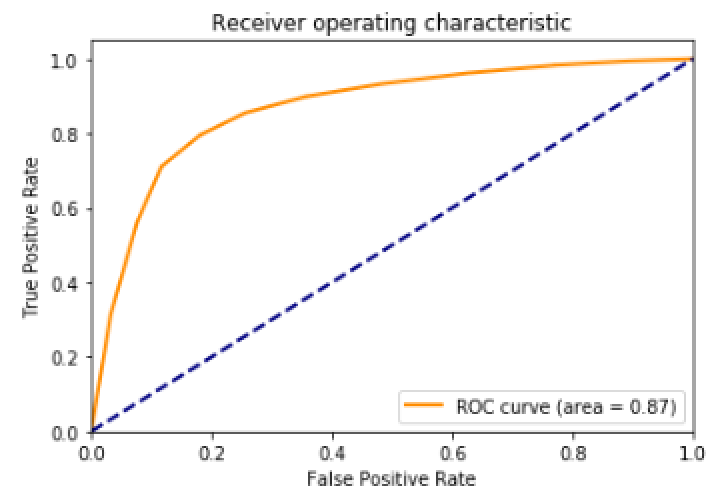
\includegraphics[width=0.5\linewidth,center] {roc1.png}
  \caption{Reciever Operator Characteristic: Pre Optimisation}
\end{figure}

Figure \ref{fig:roc1} shows the receiver operator characteristic together with the area under the curve, for the model prior to optimisation. We will track the changing shape of this graph through the various model optimisation stages.

\section{Feature Selection}
Features in ML is a term used to represent the inputs for a model that are used to predict the target variable. In the model, features include explanatory variables and our target is the variable that the model is trying to predict. We are working with a binary classifier so our target has the labels positive or negative. It is important to choose the right features as they are the key driver behind model performance. A common selection processes is to use statistical correlations to pick out the features that have a statistically significant relationship with the target. We may then choose to fit all these statistically significant features to the model and experiment with their removal until the optimum performance is achieved. Typical correlation measures include Chi Squared, Pearson and Spearmans rank. Care needs to be taken when using each of these correlation measures and will need to reflect not only the data type of both the features and target but also the correlation type we wish to check. In general for categorical data we wish to use a chisq test. For non-numeric data we wish to use either Pearson or Spearman. If we suspect linear correlations use Pearson, in non-linear we will use Spearmans as this uses ordinal values rather than actual values. Our features are a mixture of categorical and continuous types whilst our target is a categorical type. To begin with we use the chisq test on our categorical features and target. 

\subsection{Chi Squared Test}

This test is is appropriate for categorical data and can be used for three types of comparisons: goodness of fit, homogenity and independence. In feature selection we will test for independence; if an explanatory variable is independent of the target variable then its fair to not include the feature in the model.The chisq stat is calculated from a data sample's contingency table and the formula:

\begin{equation}\label{chi}
{\chi_m}^2=\sum_{k=1}^{n} \frac{(O_k - E_k)^2}{E_k}
\end{equation}

where $m$ is the degrees of freedom, $O_k$ is the observed count of the variable under test in cell $k$, $E_k$ is the expected count of the variable under test in cell $k$ and $n$ is total number of cells in the table. Note that in practice we can make use of the scippy stats module which has the ability to compete chisq stats with ease.  This test statistic is used to determine suitable p-values, for suitably small p-values we reject the null hypothesis that the variable under test is independent of the target. Those features for which we are able to reject the null hypothesis are those that should be included in an initial model. Note that the chisq test has some key assumptions which are:
\begin{enumerate}
	\item Data size is sufficently large
	\item Observations are independent
	\item The expected frequency in each cell is at least $1$
\end{enumerate}

The first of these two assumptions have been met, the third has required some data manipulation to bin some of the feature labels into an other 'bucket'. Interestingly after meeting this assumption the model AUC score improved to 0.8704. It also resulted in a reduction in model features from 4324 to 234. Note that we have not yet analysed the statistical significance of the numerical features, this is complex as we would need to measure the relationship between a continuous feature and a categorical target. For simplicity we add all the numeric features to our list of features to be included in the model. It is at this point that we would usually iterate through the features that we have identified and experiment with their model inclusion in an iterative manner and interpret their impact upon the AUC score. This is an expensive task which we will revisit in parallel with Dask.


\section{Balancing the model training data}

There are a number of problems that arise in ML when data is imbalanced. Imbalance occurs when the proportion of one class label is considerably higher than the label of another class. Due to the imbalance a model may be unable to pick up the underlying patterns in the data, which can introduce bias. In our case, for the  model there is a slight imbalance as 70\% of incidents result in a positive, 30\% in a negative. There are a number of techniques which we can apply to our training data to attack this and we discuss the performance of random and more intelligent balancing methods.

\subsection{Random Sampling}
Random balancing techniques have little intelligence and choose rows at random to be deleted or duplicated, to arrive at a desired ratio between the majority and the minority class. For our data, the random over sampling method achieves the highest AUC score when the minority class is oversampled to a ratio of 70\%. The minority class, negative, increased by 70 \% and the AUC score on test is 0.8727. The random under sampling method achieves the highest AUC score when the majority class is under sampled by 60\%. The majority class, positive, decreased by 60\% and the AUC score on test is 0.8751. It seems that from a random perspective, the under sampling technique is preferred and so we now consider an alternative under sampling technique.

\subsection{Tomek Link Reduction}
Tomek link methods remove data instances that have Tomek links. These links are defined as data of different classes which are nearest neighbours of each other, so for two samples of data x and y each of a different class and any data sample z, there is a Tomek Link between x and y if:

\begin{equation}\label{distance}
 d(x,y) < d(x,z) \text{ and } d(x,y) < d(y,z)
 \end{equation}
 
 where $d(.)$ represents the distance function. When applying this idea to training data, the instances which are positive and nearest neighbours with samples of opposing negative class, will be removed from the data. Note with Tomek Link removal we have the choice to either remove 'majority' links or 'all' links. After removing 'majority' links the AUC score on test is 0.8730. Our sampling experiments have indicated that applying random under sampling and Tomek link removal have the greatest impact upon the AUC. For this reason we take through these two training data frames as $ru\_train$  $tl\_train$ through to further optimisation stages.

\section{Hyper-Paramater Tuning}
In a machine learning algorithm, we can consider two classes of parameters which are parameters and hyper-parameters. In the case of the  model, which is using a Random Forest, it’s parameters are those which are learned through the model training, these are the features and thresholds used to split at the root and internal nodes. The hyper-parameters are those that are specified before the training process begins and include the number of trees, the tree depth, the minimum samples to split, \ldots In practice the best hyper-parameters are determined by using an experimental approach rather than theory and we run the model through various combinations of hyper-parameters that maximise the AUC score subject to some cross validation. Tweaking the hyper-parameters can help achieve slight benefits in performance, but due to the high number of combinations possible it requires high computing power. We discuss the optimal combinations for:

\begin{enumerate}

\item The n\_estimators: the number of trees in the forest. I.e the number of voters. A higher number of trees will generally increase accuracy but this results in slower performance and can lead to overfitting
\item  The criterion: how to measure the quality of the split and can be either entoropy or gini to measure the quality of the split
\item The max\_depth: how deep do we want the trees to be? Trees which are too deep could be prone to overfitting. Trees which are to shallow may not learn the data well
\item The min\_samples\_split: minimum number of samples required to split a node
\item The min\_samples\_leaf: minimum number of samples required to be at a leaf node. A smaller leaf sample size may lead to the algorithm capturing noise in the data
\item The max\_features: the number of features to consider at the root and internal nodes when looking for the best split. Note that increasing the max\_features at the nodes does not always result in better performance as it may result in trees which have little diversification. The diversification of trees is a key benefit for the random forest
\item The max\_leaf\_nodes: how many leaves at the end of the trees
\item The bootstrap: if false then the whole dataset is used when building each tree. If true then bootstrap samples are used with replacement to train the trees.
\end{enumerate}

To find the optimal hyper-parameters, we complete a random grid search and then a full grid search. 
Our random grid search has the parameters:
\begin{lstlisting}[language=Python]
random_grid = { 'bootstrap' :  [True,False],
		'criterion' : ['gini','entropy'],
		'max_depth' : [20,30,40],
		'max_features' : ['auto','sqrt'],
		'min_samples_leaf' : [1,2,4 ],
		'min_samples_split' : [2,5,10,20],
		'n_estimators': [500,1000,1500,2000]}
\end{lstlisting}

The final grid search shows that the optimal parameters using $tl\_train$ and $ru\_train$ are:
\begin{lstlisting}[language=Python]
tl_best_paramaters = {  'bootstrap' :  False,
			'criterion' : 'entropy',
			'max_depth' : 25,
			'max_features' : 'sqrt',
			'min_samples_leaf' : 2,
			'min_samples_split' : 10,
			'n_estimators': 1700}
\end{lstlisting}

\begin{lstlisting}[language=Python]
ru_best_paramaters = {  'bootstrap' :  False,
			'criterion' : 'entropy',
			'max_depth' : 25,
			'max_features' : 'sqrt',
			'min_samples_leaf' : 2,
			'min_samples_split' : 12,
			'n_estimators': 500}
\end{lstlisting}
It should be noted that the best parameters were not always consistent. In fact, 'bootstrap' sometimes seemed to prefer True, other times preferred False. The n\_estimators also showed variance in its preference between $500$ to $1500$.
Regardless, using their respective indicated best parameters and training data, the Tomek Link method achieved an AUC of $0.8897$ on test whilst the Random Under Sampler achieved an AUC of $0.8893$. It would appear that the there is very little difference in performance from these two balancing techniques.

\section{Model Evaluation}

We have achieved models which have demonstrated an increase in their AUC of 2\% which is reasonable. However we are not yet done, as we have only explicitly evaluated our model performance on test data. Whilst these scores appear acceptable, we have yet to consider the bias and variance that are present in each of the models.  A model that has a high level of bias, is most likely under fit, and has not picked up the patterns in the underlying data. This means that when the model sees new data it is consistently predicts the target poorly. A model that has a high level of variance, is most likely overfit, and has picked up the patterns in the training data to well. This means that when the model sees new data it is unable to generalise well and leads to inconsistent predictions. We can interpret the levels of bias and variance in a model by comparing the model performance on the training dataset with the performance on a test dataset. In general if:
\begin{equation}
\begin{split}
&score(\text{training data}) > score(\text{test data}) \Rightarrow \text{ high variance and possibly overfit}\\
&score(\text{training data}) \approx score(\text{test data}) \Rightarrow \text{ balance between bias and variance}\\
&score(\text{training data}) < score(\text{test data}) \Rightarrow \text{ high bias and possibly under fit}\\
\end{split}
\end{equation}

The following Table \ref{tab:table1} shows the performance of the Tomek Link process and the Random Under Sampler on their respective training and testing data.
\begin{table}[h!]
  \begin{center}
    \label{tab:table1}
    \begin{tabular}{l|S|S} 
      \textbf{Modelling data} & \textbf{Tomek Link AUC} & \textbf{Random Under Sampler AUC}\\
      \hline
       Train* & 0.9826 & 0.9800\\
      Test & 0.8897 & 0.8893\\
    \end{tabular}
  \end{center}
  \caption{AUC score for Tomek Link and Random Under Sampler on train and test (hyper-parameters)}
\end{table}

Note that Train* indicates the respective training sets for each of the Tomek Link and Random Under Sampler methods. From equation \ref{tab:table1} we see that both methods have performed considerably better on the training data than on the test data. This indicates that both are displaying high levels of variance and so are overfit. We see that the Tomek Link process has achieved a higher AUC on the test data but this than the Random Under Sampler, but also with a higher performance difference when compared to test. This may suggest that either for the balancing method used, or the hyper-parameters that were optimised for, the TL model is displaying higher levels of variance. That being said, the differences between these two process seems fairly small. It is worth us now choosing a set of hyper-parameters, based on the results of the grid search, that may be less prone to over fitting like:

\begin{lstlisting}[language=Python]
less_overfit_parameters = {bootstrap= True,
			 max_depth= 20,
			 max_features= 'sqrt',
			 min_samples_leaf=15,
			 min_samples_split= 30,
			 n_estimators= 500,
			 criterion='entropy')
\end{lstlisting}

Table \ref{tab:table2} shows the performance of the Tomek Link process and the Random Under Sampler on their respective training and testing data, but with parameters less prone to over fitting.
\begin{table}[h!]
  \begin{center}
    \label{tab:table2}
    \begin{tabular}{l|S|S} 
      \textbf{Modelling data} & \textbf{Tomek Link AUC} & \textbf{Random Under Sampler AUC}\\
      \hline
       Train* & 0.9177 & 0.9143\\
      Test & 0.8868 & 0.8867\\
    \end{tabular}
  \end{center}
    \caption{AUC score for Tomek Link and Random Under Sampler on train and test (softer-parameters)}
\end{table}

We can see that by choosing these softer parameters our train scores are now closer to the test scores and this seems an acceptable difference. There is very little evidence to separate the two balancing methods. It seems that the Tomek Link method may be slightly more prone to overfitting than the random under sampler when the same parameters are used. The following Figure \ref{fig:roc2} shows the ROC curve for the two balancing approaches when the same parameters have been used.

\begin{figure}[h]\label{fig:roc2}
  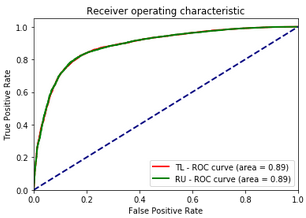
\includegraphics[width=0.5\linewidth,center] {roc2.png}
  \caption{Reciever Operator Characteristic: Post Optimisation}
\end{figure}

Their appears to be little separation between the two curves.  It seems that the balancing method does not seem to have a significant impact upon model performance. Regardless of the balancing method, through the optimisation stages, we have managed to achieve an increase in AUC of 2\%. Subsequent work will consider, iterative feature selections and comparisons from the Random Forest to the Gradient Boosting algorithms. 



















































































































\end{document}
